\Lecture{Princy Lunawat}{Jan 25, 2012}{11}{Amplification Lemma}

In the last lecture, we saw the polynomial identity testing problem
and a randomized algorithm for it. We also discussed how branching machines with
guarantees on the number of erroneous paths characterize randomized
algorithms. We ended the last lecture with a question about how two
sets of languages compare. $\BPP_{\epsilon}$ and $\BPP_{\epsilon'}$.
for different $\epsilon$ and $\epsilon'$? 

\section{Amplification of Success Probability}

We showed that if $\epsilon < \epsilon'$ then $\BPP_{\epsilon} \subseteq \BPP_{\epsilon'}$. A strategy to prove the other direction was the following : Repeat the randomized algorithm (experiment) multiple
times (say $k$), and then take the majority of the outcomes in order to improve our success probability.
One remark is that the repetition is sequential and happens on each
branch. Thus we are essentially producing a new branching machine with
many deeper computation paths. 

Why would this improve the success probability? and if so, how does it depend on $k$?. 
The following lemma answers these.

\begin{lemma}
If $\mathcal{E}$ is an event that $Pr(\mathcal{E}) \geq \frac{1}{2} + \epsilon $, then the probability the $\mathcal{E}$ occurs atleast $\frac {k}{2}$ times on $k$ independent trials is at least 
$1-\frac{1}{2}(1-4\epsilon^2)^\frac{k}{2}$
\end{lemma}
\begin{proof}
Let $q$ denote the probability the $\mathcal{E}$ occurs atleast $\frac {k}{2}$ times on $k$ independent trials.
Let $q_i$ = Pr($\mathcal{E}$ occurs exatly $i$ times in $k$ trials), $0 \leq i \leq k$. Thus,
$q = 1 - \sum_{i=0}^{\lfloor\frac{k}{2}\rfloor}$ $q_i$. We will analyse the complementary event:
Pr($\mathcal{E}$ occurs atmost $\frac{k}{2}$ times) = $\sum_{i=0}^{\lfloor\frac{k}{2}\rfloor}$ $q_i$. \\ 
We show an upper bound on each $q_i$ and thus show an lower bound on $q$.
\begin{eqnarray*}
q_i & = & {k \choose i} (\frac{1}{2} + \epsilon)^{i} (\frac{1}{2} - \epsilon)^ {k-i} \\
& \leq & {k\choose i} \left(\frac{1}{2} + \epsilon\right)^{i} \left(\frac{1}{2} - \epsilon\right)^ {k-i} \left(\frac{\frac{1}{2} + \epsilon}{\frac{1}{2} - \epsilon}\right)^{\frac{k}{2} - i}  (because \epsilon \le \frac{1}{2} ) \\
& = & {k\choose i}\left(\frac{1}{2} + \epsilon\right)^{\frac{k}{2}}\left(\frac{1}{2} - \epsilon\right)^{\frac{k}{2}} \\
&= & {k\choose i} \left(\frac{1}{4} - \epsilon^2\right)^{\frac{k}{2}}
\end{eqnarray*}
Now we analyse the sum:
\begin{eqnarray*}
\sum_{i=0}^{\lfloor\frac{k}{2}\rfloor}q_i & \leq & \sum_{i=0}^{\lfloor\frac{k}{2}\rfloor}{k\choose i} \left(\frac{1}{4} - \epsilon^2\right)^{\frac{k}{2}} \\
q = 1 - \sum_{i=0}^{\lfloor\frac{k}{2}\rfloor}q_i & \geq & \sum_{i=0}^{\lfloor\frac{k}{2}\rfloor}{k\choose i} \left(\frac{1}{4} - \epsilon^2\right)^{\frac{k}{2}} \\
& = & 1 - \left(\frac{1}{4} - \epsilon^2\right)^{\frac{k}{2}} 2^{k-1} \\
& = & 1 - \frac{1}{2} \left(1 - 4\epsilon^2\right)^{\frac{k}{2}} \\
\textrm {Thus, } q & \ge & 1 - \frac{1}{2} \left(1 - 4\epsilon^2\right)^{\frac{k}{2}}
\end{eqnarray*}
\end{proof}

In the last lecture, we defined the class $\BPP_\epsilon$ (Bounded Error Probabilistic Polynimial Time) and now we can use the above amplification lemma to prove that
\[\BPP_{\epsilon} = \BPP_{\epsilon^{'}} \hspace{3mm}\forall  0 \leq \epsilon , \epsilon' < \frac{1}{2} \]

We want to calculate
In general, the above lemma can be used to prove that , at the cost of running time, the the error probability of a language $L$ , 
$L \in \BPP$ can be reduced to $\frac{1}{2^{q(n)}}$ where $q(n)$ is a polynomial in $n$.
 
\begin{lemma}
$L \in \BPP$ if an only if for any polynomial $q(n)$ there is a machine $M$ that runs for time $p(n)$ (which depends on $q(n)$) such that \\
\[ \textrm{ Pr($M$ errs on input $x$)) } \le 2^{-q(n)} \] 
In terms of number of paths,
\[ \#err_M(x) \le  2^{p(n)-q(n)} \]
\end{lemma}
\begin{proof}
Given a language $L \in \BPP_\epsilon$ with PTM $M$, we design a PTM $N$ such that $L(N) \in \BPP$ and $L(n) = L$ as follows:
\begin{itemize}
 \item Run the machine $M$ on input $x$ $k$ times independently where choice of $k$ is such that
\\
\begin{equation}\label{eq:eq2}
 \frac{1}{2} \left(1 - 4\epsilon^2\right)^{\frac{k}{2}} \leq 2^{-q(n)}
\end{equation}

\end{itemize}
The above equation $\eqref{eq:eq2}$ yields a value of $k$ polynomial in $n$ and hence $N$ runs a polynomial number of times.
The amplification lemma ensures that the error probability reduces to the LHS of the equation $\eqref{eq:eq2}$.
\end{proof}

\section*{The Structure of \BPP}
We explore some interesting structural properties about the class $\BPP$.

\begin{proposition}
$\BPP$ is closed under complementation.
\end{proposition}
\begin{proof}
Let $L \in BPP$ via PTM $M$ with error probability $\epsilon < \frac{1}{2}$ . We show that $\bar L$ is in $\BPP$.
We design a new machine $\bar M$ by switching the accept and reject states of $M$.
\begin{eqnarray*}
x \in L & \implies & \#acc_M(x) \geq (1 - \epsilon )\#path_M(x) \\
& \implies & \#rej_M(x) \leq \epsilon \#path_M(x). \\
& \implies & \#acc_{\bar M} \leq \epsilon \#path_{\bar M}(x). \\
& \implies & x \notin L(\bar M). \\
x \notin L & \implies & \#acc_M(x) \leq \epsilon.\#path_M(x). \\
& \implies & \#rej_M(x) \geq (1-\epsilon)\#path_M(x). \\
& \implies & \#acc_{\bar M} \geq (1-\epsilon) \#path_{\bar M}(x).\\
& \implies & x \in L(\bar M).
\end{eqnarray*}

Hence, we have,
\[x\in L \iff x\notin L(\bar M) \]
Therefore, $L(\bar M) = \bar L$ and $L \in BPP$ via machine $\bar M$. Hence,
$BPP$ is closed under complementation.
\end{proof}

%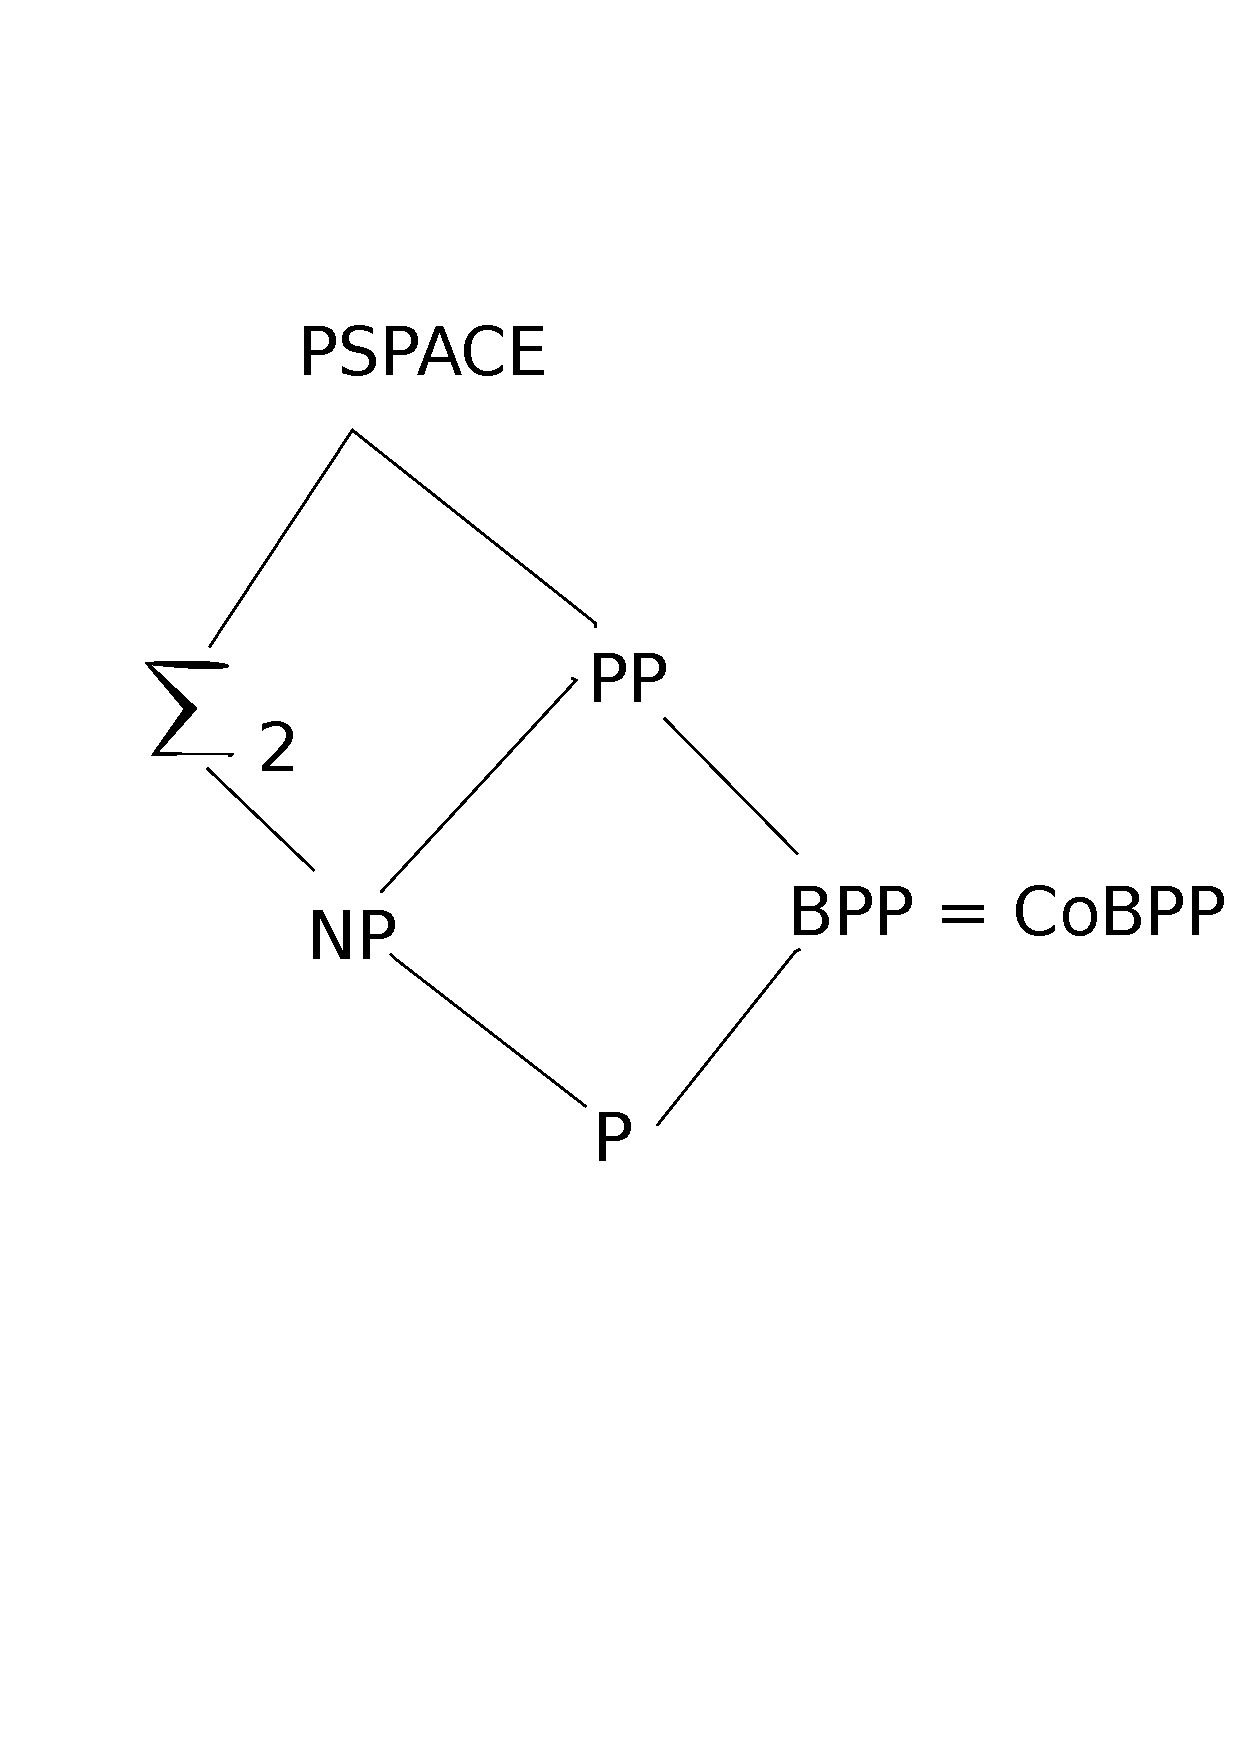
\includegraphics[scale=0.5,trim = 10mm 80mm 50mm 5mm]{hie1}
%\pagebreak

\section*{One-sided Error Randomized Algorithms}

Consider the language , PIT that is, Polynomial Identity Testing,
\[PIT =\{ p |  p\equiv 0 \}\] where $p$ is a polynomial.
From, the last lecture, we make the following observation about PIT,
if $p \in PIT$, PTM makes no error,
if $p \notin PIT$, PTM makes some error (less than half the number of paths).

We now explore how complexity theory can be extended to these kind of algorithms too.
\begin{definition}({\bf \RP})
A language $L$ is said to be in $\RP$ if there is an $\epsilon$ such
that $0 < \epsilon < \frac{1}{2}$, and a randomized algorithm $A$ such that :
\begin{eqnarray*}
x \in A & \implies & Pr [\textrm{ $A$ accepts }] \ge \frac{1}{2}+\epsilon \\
x \notin A & \implies & Pr [\textrm{ $A$ accepts }] = 0
\end{eqnarray*}
\end{definition}

Hence we have the following proposition:
\begin{equation}
PIT \in \co\RP
\end{equation}

\begin{proposition}
$\RP \subseteq \NP$
\end{proposition}
\begin{proof}
Consider language $L \in \RP$ via machine $M$ such that 
$x \in L \implies M $ accepts $x$ with some error $\epsilon < \frac{1}{2}$
$\implies M $ accepts $x$ on atleast 1 path. \\
$x \notin L \implies M$ accepts $x$ with probability 0 $\implies M$ rejects on all paths.
Thus $L \in \NP$. Moreover, even with the acceptance condition of a non-deterministic machine, the branching machine corresponding to the $\RP$ algorithm accepts the language $L$ itself.
\end{proof}
\vspace{-40mm}
\begin{center}
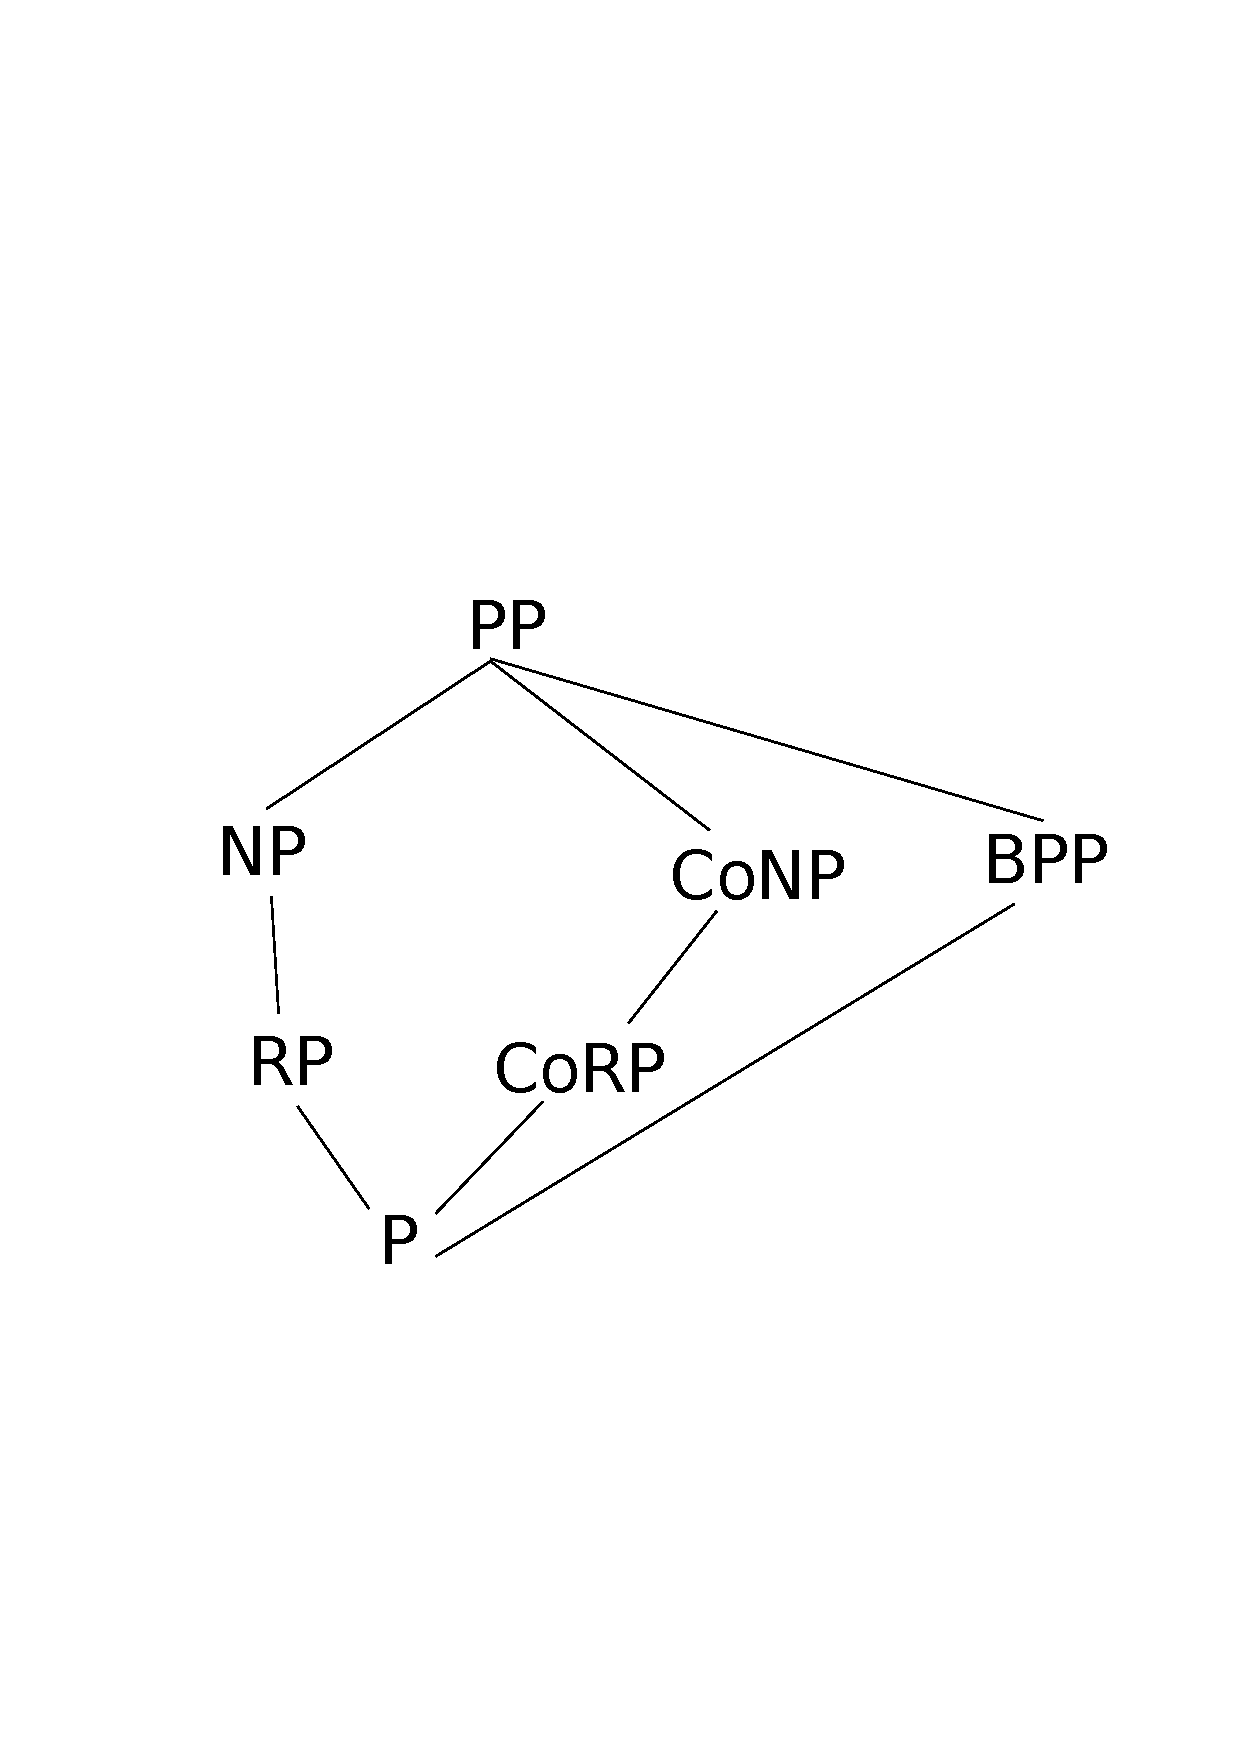
\includegraphics[scale=0.3, trim = 30mm 50mm 0mm 5mm, clip]{Lecture11-Princy/hie2}
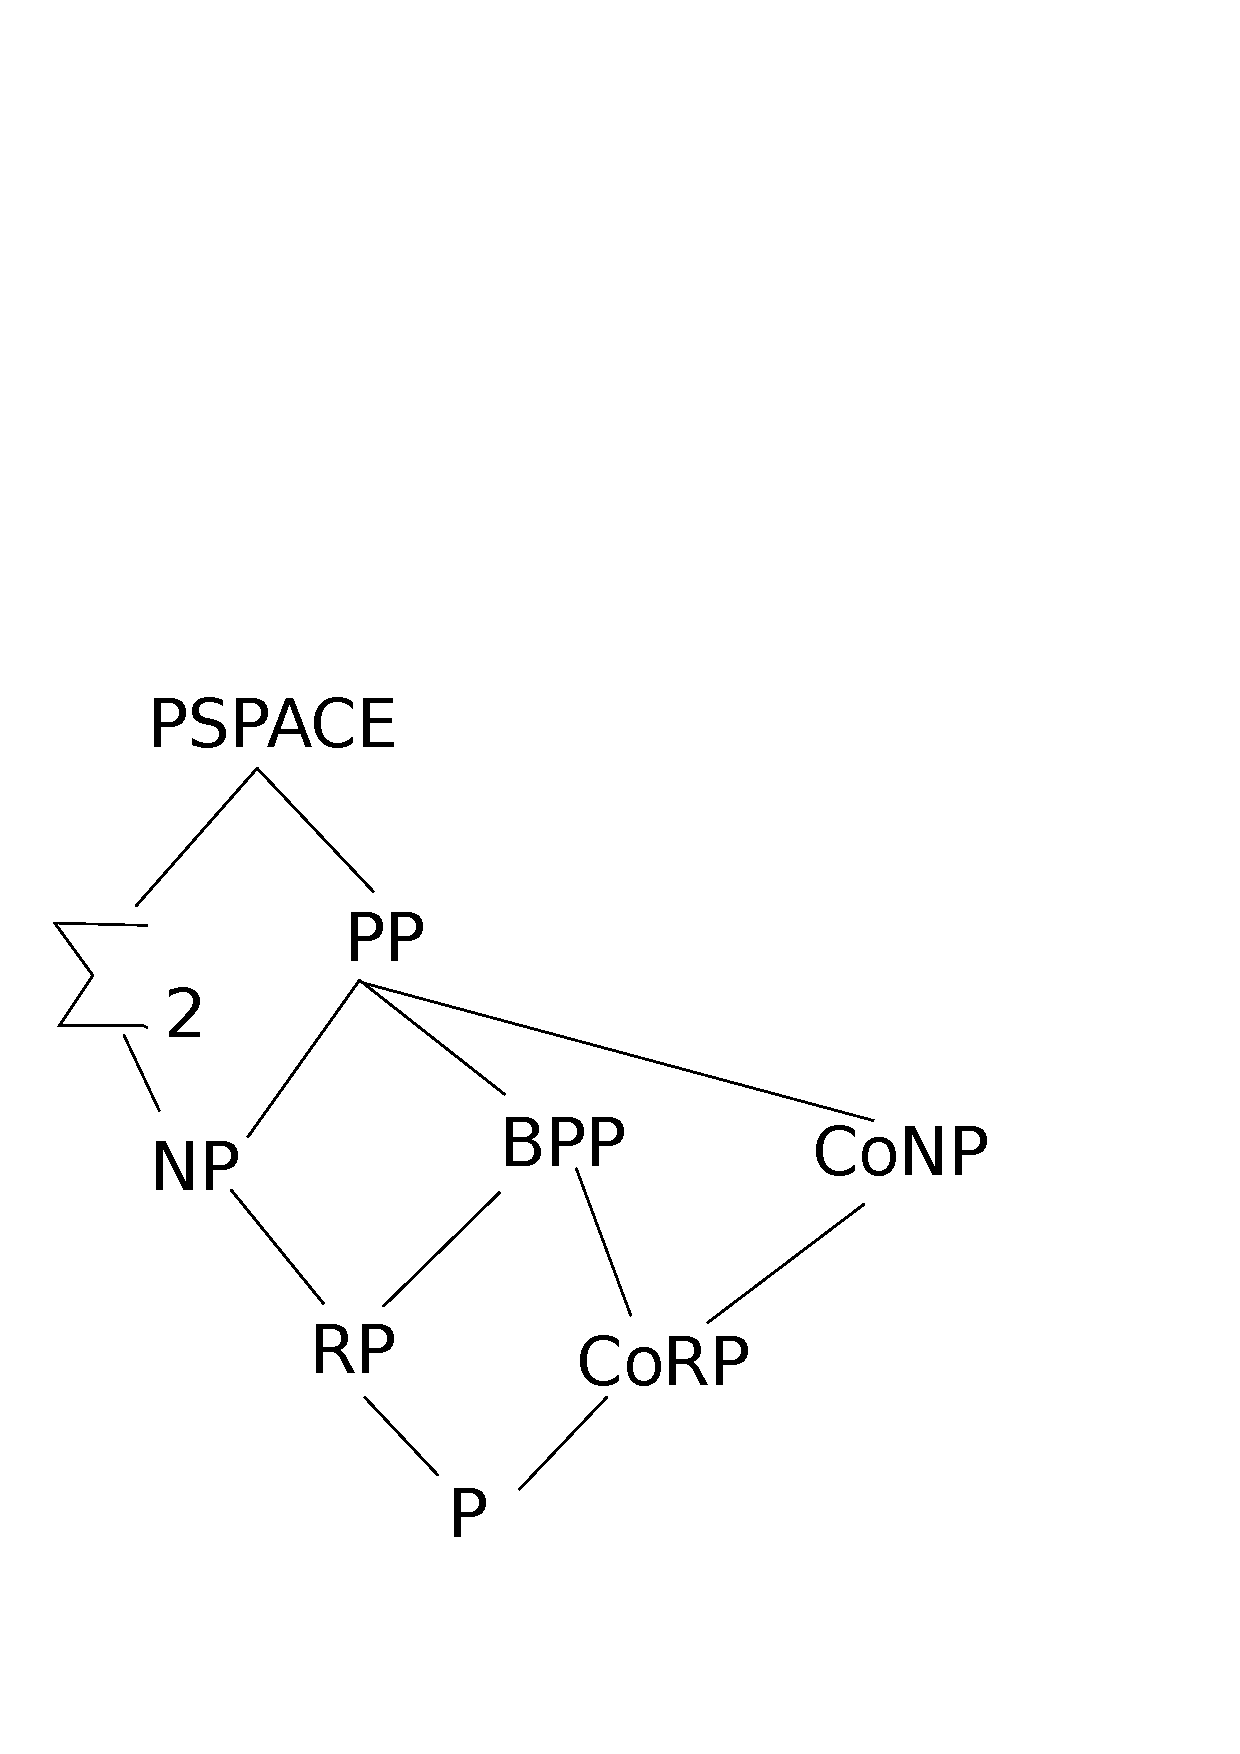
\includegraphics[scale=0.3]{Lecture11-Princy/hie3}
\end{center}
\vspace{-10mm}

\section{Derandomization of $\BPP$}
There are several questions connected to the new class $\BPP$ that contains several natural problems. We saw one example of multivariate polynomial identity testing problem. Is $BPP \subseteq P$? This would amount to showing that in the world of efficient computations, randomization does not add any power. There are reasons to remotely believe this to be the case, but till date there is no proof. 

A question of slightly different flavour is, if problems in $\BPP$ are contained in $\NP$? That is, can we trade non-determinism with randomness? We already know that if the randomness causes only one-sided error, then it can be replaced by simple non-deterministm ($\RP \subseteq \NP$). But extending this to two-sided error version is an interesting open problem in the area. 

We show a relaxed containment which can be seen to be an improved upper bound for problems in $\BPP$ compared to the trivial upper bound of $\PSPACE$.

\begin{theorem}
$BPP \in \Sigma_2$
\end{theorem}
\begin{proof}
Let $L \in \BPP$. By using amplification lemma for $q(n) = n$ we can state:
there is a probabilistic Turing machine $M$ and polynomial p(n) such that,
\[\#err_M(x) \leq 2^{-n} 2^{p(n)}\]

Let us recall the definition and a characterization of the class $\Sigma^2$
$\Sigma_2$ is defined as follows:
$L \in \Sigma_2$ iff $\exists B \in P $ such that:
\[x \in L \iff \exists y,  \forall z,  (x,y,z) \in B\]

There is a clear mindblock here. How do we tradeoff quantifiers to randomness?

Let us define a set A(x) as follows:
\[ A(x) = \{y\in \{0,1\}^{p(n)} |  M\ accepts\ x\ on\ path\ y \}\]

Observe that, 
\[x \in L \Rightarrow |A(x)| \geq (1- 2^{-n}) 2^{p(n)} \]
that is, no. of $y$'s such that $M(x,y) = 1$ is large.
\[x \notin L \Rightarrow |A(x)| \leq  2^{-n} 2^{p(n)}) \] 
that is, no, of $y$'s such that $M(x,y) = 1$ is small.
\\

\textbf{Parity Map:}
For two strings $y,z \in \{0,1\}^{p(n)}$, let $y \parity z$ denote the bit-wise parity of the two strings.
We can extend the parity map to operate on subsets of $\{0,1\}^{p(n)}$ as follows:
\[ S \parity z = \{y \parity z ~|~ y \in S \, z \in \{0,1\}^{p(n)} \}\]

\begin{observation}
For a fixed $z$, $\parity_z$ is a bijection from $\{0,1\}^{p(n)} \to \{0,1\}^{p(n)}$. That is, for any $z \in \{0,1\}^{p(n)}$, and $S \subseteq \{0,1\}^{p(n)}$, $|S| =|S \parity z|$.
\end{observation}

Ask the question : how many $z$'s do we need to cover $\{0,1\}^{p(n)}$ entirely?
That is, how large do we need $m$ to be, such that there exists strings $z_1, z_2, \ldots, z_m$ such that:
\[\bigcup_{i=1}^{m} (A(x) \parity z_i) = \{0,1\}^{p(n)}  \]

Intuitively, we expect the answer to be {\em small} when the size of $A(x)$ is large, and {\em large} when the size of $A(x)$ is small. Now we formalize this.

\textbf{Case 1:} Small $|A(x)| \leq 2^{-n} 2^{p(n)}$
In the best case, let each $z_i$ maps $A(x)$ to non-intersecting sets.
\[ \forall i, j (A(x)\parity z_i) \cap (A(x) \parity z_j) = \phi , i \neq j \]
\[|\bigcup_{i=1}^{m} (A(x) \parity z_i)| \geq |\{0,1\}^{p(n)}|\]
\[\Rightarrow m (2^{-n}) 2^{p(n)} \geq 2^{p(n)}\]
\[\Rightarrow m \geq 2^n\]

Hence, the no. of $z$'s required is exponential in $n$ when $A(x)$ is small, that is, when
$x \notin L$.
\\

\textbf{Case 2:} Large $|A(x)| \geq (1 - 2^{-n}) 2^{p(n)}$
We prove that $\exists z_1, z_2, z_3 ... z_m$ for a small $m$ such that 
\[|\bigcup_{i=1}^{m} (A(x) \parity z_i)| = |\{0,1\}^{p(n)}|\]
We call the $m$-tuple $z_1, z_2, z_3 ... z_m$ {\em bad}, if ,
\[|\bigcup_{i=1}^{m} (A(x) \parity z_i)| \neq |\{0,1\}^{p(n)}|\]
\[\Rightarrow \exists w \in \{0,1\}^{p(n)}, z_i \parity y \neq w ,\forall y \in
A(x), \forall i \]
\[\Rightarrow \{z_i \parity w | 1 \leq i \leq m \} \subset R(x)\]
where $R(x) = \bar A(x)$.
$|R(x)| = 2^{p(n)} - |A(x)|$
$\Rightarrow |R(x)| \leq  2^{p(n) - n}$

For a given $w$ and a given subset of $R(x)$ of size $m$, we get a {\em bad} $m$-tuple
$z_1, z_2, z_3 ... z_m$. Hence,
\\
Number of {\em bad} $z_1, z_2, z_3 ... z_m \leq $ Number of of $w$'s $\times$ Number of subsets
of $R(x)$ of size $m$.
\\
$\Rightarrow$ Number of {\em bad} $z_1, z_2, z_3 ... z_m \leq 2^{p(n)} (2 ^{p(n)-n})^m $
\\
Total number of $z_1, z_2, z_3 ... z_m $ = $(2^{p(n)})^m$.
$m$ should be such that,
\[2^{p(n)} (2 ^{p(n)-n})^m < (2^{p(n)})^m\]
\[p(n) + (p(n)-n)m < p(n)m\]
\[p(n) - nm < 0\]
\[m > \frac{p(n)}{n}\]

This goes well with our intuition. If $m$ is allowed to be very small, then we should not be able to cover the entire set $\{0,1\}^n$. For, $m > \frac{p(n)}{n}$ we are guaranteed to have atleast one {\em good} $m$-tuple, that is,
\[z_i \parity w = y , y \in A(x)\]

Hence we conclude that, 
\[\exists z_1, z_2, z_3 ... z_m , \forall w \in \{0,1\}^{p(n)} \left( \bigwedge_{i=1}^{m} \left[~z_i \parity w
\in A(x) ~\right] \right) \]
\[\exists z_1, z_2, z_3 ... z_m , \forall w \in \{0,1\}^{p(n)}, \left( \bigwedge_{i=1}^{m} \left[ ~M(x, z_i
\parity w) = 1 ~\right] \right) \]

Checking if $M$ accepts $x$ on a given path is a polynomial time operation, and
repeating it for each $z_i$ where the number of $z_i$'s is polynomial in $n$ is
also a polynomial time operation. Fix $m = p(n)$, Thus we have a $B \in \P$ such that

\[ x \in L \iff \exists \overline{z} \in \{0,1\}^{p(n)^2}, \forall w \in \{0,1\}^{p(n)} (x,\overline{z},w) \in B \]
Hence, the above language $L \in \Sigma_2$.
\end{proof}
  
